\documentclass[10pt,letterpaper,twoside]{article}
\usepackage{code/manuscript_assets/researchpreprint}
\usepackage[T1]{fontenc}
\usepackage{lmodern}
\usepackage{microtype}
\usepackage{amsmath,amssymb,amsthm}
\usepackage{booktabs}
\usepackage{tabularx}
\usepackage{graphicx}
\usepackage{caption}
\usepackage{float}
\usepackage{xurl}
\usepackage[numbers,sort&compress]{natbib}
\usepackage[hidelinks]{hyperref}

\newtheorem{theorem}{Theorem}
\newtheorem{corollary}[theorem]{Corollary}
\newtheorem{proposition}[theorem]{Proposition}
\newcommand{\R}{\mathbb{R}}
\newcommand{\norm}[1]{\left\lVert #1\right\rVert}

\title{Station-Referenced Streaming Energy Ratios for Early
Ground-Motion Screening}
\author{Molena Huynh}
\email{molena.huynh@jmp.com}
\affiliation{North Carolina State University}
\date{}

\hypersetup{
  pdftitle={Station-Referenced Streaming Energy Ratios for Early Ground-Motion Screening},
  pdfauthor={Molena Huynh}
}

\begin{document}
\setlength{\emergencystretch}{2em}
\maketitle

\begin{abstract}
A compact covariance approximation is not useful for ground-motion screening
if physical amplitude already carries the dominant class information.  We
replace a rejected butterfly-whitening model by a streaming statistic that
retains amplitude and removes station-scale variation with a checksum-verified
historical reference.  Three-component velocity samples are centered within
3.2-second blocks.  The statistic after $k$ blocks is the base-10 logarithm
of the candidate prefix mean energy divided by the reference-window mean
energy.  The development rule chooses the prefix from
$\{3.2,6.4,12.8,25.6,51.2,102.4,204.8\}$ seconds that maximizes
leave-one-earthquake-out balanced accuracy, with shorter latency resolving a
tie.  It selects 25.6 seconds and fixes the threshold before confirmation.

The study contains 108 original EarthScope FDSN responses, 66.98 MB in total,
linked to twelve magnitude-8.0 or larger USGS events.  Eight events and six
stations support development.  Four later events and three previously unused
stations form confirmation; a one-day-offset trace supplies the reference and
a two-day-offset trace supplies an independent negative.  On the twelve
confirmation pairs, the proposed statistic attains balanced accuracy 0.792,
sensitivity 0.667, specificity 0.917, and area under the ROC curve 0.833 after
25.6 seconds.  Raw mean energy and the raw 0.9-energy quantile each attain
balanced accuracy 0.708 and area 0.833.  The paired bootstrap interval for the
balanced-accuracy difference is $[-0.083,0.250]$; the observed improvement is
therefore not statistically resolved.  A deterministic perturbation theorem
certifies decisions separated from the threshold, while a one-pass
implementation costs $O(ckb)$ operations and $O(c)$ numerical state for $c$
channels and block length $b$.  The measured median apply time is 56.1
microseconds at the selected prefix.  The result is an authenticated early
screening study, not an operational phase picker or a universal detector.
\end{abstract}

\begin{keywords}
streaming signal processing, station normalization, ground motion,
checksum-verified waveforms, perturbation bounds, matrix-free computation
\end{keywords}

\section{Introduction}

Seismic monitoring joins a physical signal, a station response, ambient
conditions, and a decision rule.  A representation that suppresses scale can
discard the most discriminative component of a catalog-window benchmark.
That failure occurred in the preceding covariance-whitening experiment on
EarthScope Global Seismographic Network records: no learned butterfly
candidate met its action-error certificate, and an unwhitened amplitude
control exceeded every covariance-based score.  The present work begins from
that falsification rather than from the rejected representation.

The redesigned problem concerns early screening of a fixed candidate window.
Each three-component trace is compared with a station-matched historical
quiet trace.  The comparison preserves relative amplitude while canceling a
common multiplicative station gain.  It is updated block by block, requires no
covariance matrix, and returns a scalar after each block.  The statistical
role is deliberately limited.  Established pickers and learned phase
detectors address onset localization and operational event association
\cite{allen1978automatic,ross2018generalized,zhu2019phasenet}.  Our experiment
instead evaluates catalog-window separation at a fixed 15-minute offset from
large-event origin times.

Three elements define the contribution.  First, the station-reference ratio
has an explicit gain invariance and a sharp relative-error perturbation bound.
Second, prefix length and threshold are fixed by an event-grouped development
protocol, then evaluated on later earthquakes at stations unused during
development.  Third, every waveform response is linked to its provider URL,
byte count, channel identifiers, units, and SHA-256 digest.  The new method is
not tuned after confirmation and is compared with two amplitude controls that
can defeat it.

The figures follow a claim--mechanism--cost organization.  Figure~\ref{fig:prefix}
shows the latency--accuracy relationship and the development-selected prefix.
Figure~\ref{fig:scores} exposes every confirmation score, including the four
event misses and one quiet-window false alarm.  Figure~\ref{fig:cost} compares
measured time with the constant numerical state asserted by the complexity
theorem.  The tables identify the data partitions and report task metrics
rather than decorative summaries.

\section{Station-referenced prefix statistic}

Let $X\in\R^{c\times n}$ be a candidate trace and
$Q\in\R^{c\times n_Q}$ a station-matched reference trace.  For block length
$b$, define the centered energy of candidate block $j$ by
\begin{equation}
\begin{aligned}
 e_j(X)&=\sum_{r=1}^{c}\sum_{s=1}^{b}
 \left(X_{r,(j-1)b+s}-\bar X_{rj}\right)^2,\\
 \bar X_{rj}&=\frac{1}{b}\sum_{s=1}^{b}X_{r,(j-1)b+s}.
\end{aligned}
 \label{eq:block-energy}
\end{equation}
If the reference contains $m_Q$ complete blocks, its fixed scale is
\begin{equation}
 \mu_Q=\frac{1}{m_Q}\sum_{j=1}^{m_Q}e_j(Q).
 \label{eq:reference}
\end{equation}
The candidate prefix statistic is
\begin{equation}
 S_k(X;Q)=\log_{10}\left(
 \frac{k^{-1}\sum_{j=1}^{k}e_j(X)}{\mu_Q}
 \right).
 \label{eq:statistic}
\end{equation}
A candidate is positive at the registered prefix $k_\star$ precisely when
$S_{k_\star}\geq\theta_\star$.

For the EarthScope records, $c=3$, $b=64$, and the sample rate is 20 Hz.
One block therefore represents 3.2 seconds.  The reference is the window one
day before the event-aligned candidate.  The negative is a distinct window
two days before that candidate; it is never reused as the denominator.

\subsection{Registered selection}

The candidate prefixes are
\begin{equation}
 \mathcal K=\{1,2,4,8,16,32,64\}.
\end{equation}
For each $k\in\mathcal K$, an entire earthquake is removed, the threshold
maximizing balanced accuracy is fit on the other seven earthquakes, and the
held-earthquake score is recorded.  The mean of the eight held-earthquake
scores is the selection objective.  Ties favor the smaller $k$.  This rule
selects $k_\star=8$, or 25.6 seconds; $k=16$ has the same mean development
score and twice the latency.  A final threshold fit to all development pairs
gives
\begin{equation}
 \theta_\star=0.8422956584.
 \label{eq:threshold}
\end{equation}
Neither $k_\star$ nor $\theta_\star$ is changed after confirmation records are
opened.

\section{Deterministic analysis}

The following statements concern the computed statistic.  They do not imply
a stochastic false-alarm guarantee for an arbitrary seismic stream.

\begin{theorem}[Common-gain invariance]
Let $a\neq0$.  For every admissible prefix,
\begin{equation}
 S_k(aX;aQ)=S_k(X;Q).
\end{equation}
\end{theorem}

\begin{proof}
Centering is linear, hence every block energy is homogeneous of degree two:
\begin{align}
 e_j(aX)
 &=\sum_{r,s}\left(aX_{r,(j-1)b+s}-a\bar X_{rj}\right)^2 \\
 &=a^2 e_j(X).
\end{align}
Likewise, $\mu_{aQ}=a^2\mu_Q$.  Substitution into
\eqref{eq:statistic} cancels $a^2$:
\begin{align}
 S_k(aX;aQ)
 &=\log_{10}\left(
 \frac{a^2 k^{-1}\sum_{j=1}^{k}e_j(X)}{a^2\mu_Q}
 \right) \\
 &=S_k(X;Q). \qedhere
\end{align}
\end{proof}

\begin{theorem}[Relative-error certificate]
Suppose the computed candidate prefix mean $\widetilde\mu_X$ and reference
mean $\widetilde\mu_Q$ satisfy, for some $0\leq\delta<1$,
\begin{equation}
 |\widetilde\mu_X-\mu_X|\leq\delta\mu_X,
 \qquad
 |\widetilde\mu_Q-\mu_Q|\leq\delta\mu_Q.
 \label{eq:relative-error}
\end{equation}
Then the exact and computed log ratios obey
\begin{equation}
 |\widetilde S_k-S_k|
 \leq
 \eta(\delta)
 :=\log_{10}\frac{1+\delta}{1-\delta}.
 \label{eq:certificate}
\end{equation}
The bound is attained when the numerator is perturbed upward and the
denominator downward, or conversely.
\end{theorem}

\begin{proof}
Inequalities~\eqref{eq:relative-error} imply
\begin{equation}
 \frac{1-\delta}{1+\delta}
 \leq
 \frac{\widetilde\mu_X/\widetilde\mu_Q}{\mu_X/\mu_Q}
 \leq
 \frac{1+\delta}{1-\delta}.
\end{equation}
Taking base-10 logarithms and absolute values proves
\eqref{eq:certificate}.  Equality follows by setting
$\widetilde\mu_X=(1+\delta)\mu_X$ and
$\widetilde\mu_Q=(1-\delta)\mu_Q$, or by reversing the signs.
\end{proof}

\begin{corollary}[Decision preservation]
If
\begin{equation}
 |S_k-\theta_\star|>\eta(\delta),
 \end{equation}
then the exact and computed statistics lie on the same side of
$\theta_\star$.
\end{corollary}

\begin{proof}
For $S_k>\theta_\star$, the premise and Theorem~2 give
\begin{equation}
 \widetilde S_k\geq S_k-\eta(\delta)>\theta_\star.
\end{equation}
The case $S_k<\theta_\star$ follows from
$\widetilde S_k\leq S_k+\eta(\delta)<\theta_\star$.
\end{proof}

Figure~\ref{fig:scores} visualizes the empirical margins
$S_{k_\star}-\theta_\star$.  It supports inspection of decision separation;
it is not a substitute for the deterministic proof.

\begin{theorem}[Streaming complexity]
For $c$ channels, block length $b$, and $k$ candidate blocks,
$S_k$ can be updated in $O(ckb)$ arithmetic operations and $O(c)$ numerical
state beyond the input block.  The reference contributes one precomputed
scalar.  A stored-vector implementation of the $k$ block energies instead
requires $O(k)$ additional storage.
\end{theorem}

\begin{proof}
For each channel and block, retain the two partial sums
\begin{equation}
 u_{rj}=\sum_{s=1}^{b}X_{r,(j-1)b+s},
 \qquad
 v_{rj}=\sum_{s=1}^{b}X_{r,(j-1)b+s}^{2}.
\end{equation}
The centered block energy is evaluated without a matrix:
\begin{equation}
 e_j(X)=\sum_{r=1}^{c}\left(v_{rj}-\frac{u_{rj}^{2}}{b}\right).
\end{equation}
Computing $u_{rj}$ and $v_{rj}$ costs $O(cb)$ operations.  Adding $e_j$ to a
single running energy sum costs $O(1)$, so $k$ blocks cost $O(ckb)$.  The
partial sums occupy $O(c)$ scalars and are reused; the block counter,
accumulated energy, and reference mean require $O(1)$ additional state.
Storing all $e_j$ values uses $k$ scalars and therefore $O(k)$ storage.
\end{proof}

\section{Authenticated waveform study}

\subsection{Sources and partitions}

Event identifiers and metadata come from the USGS ComCat service
\cite{usgs2026comcat}.  Waveforms come from the EarthScope FDSN data-select
service for the IU Global Seismographic Network
\cite{iu1988network,earthscope2026gsn,earthscope2026fdsn}.  Each request asks
for location 00 and the three BH components, with provider scaling retained
in meters per second.  Components are interpolated to their common 20-Hz
grid only after a gap and coverage check.

The study uses 108 original responses totaling 66,981,395 bytes.  Every
response is represented in the locked result by its URL, SHA-256 digest,
byte count, channel identifiers, scale units, and common sample count.  No
waveform is redistributed.  Table~\ref{tab:data} separates development and
confirmation by both earthquake and station.

\begin{table}[H]
\centering
\caption{Authenticated data partitions.  A pair comprises one event-aligned
candidate, one one-day reference, and one independent two-day negative.}
\label{tab:data}
\small
\begin{tabularx}{\columnwidth}{@{}lXXr@{}}
\toprule
Role & Earthquakes & Stations & Pairs \\
\midrule
Development
& Maule, Tohoku, Wharton, Okhotsk, Iquique, Illapel, Tehuantepec, Peru
& ANMO, COLA, MAJO, COR, KONO, HRV
& 24 \\
Confirmation
& Kermadec, Chignik, South Sandwich, Kamchatka
& TATO, PAB, CASY
& 12 \\
\bottomrule
\end{tabularx}
\end{table}

The development events span 2010--2019.  The confirmation events span
2021--2025 and have magnitudes 8.1, 8.2, 8.1, and 8.8.  Candidate windows
begin 900 seconds after catalog origin and last 240 seconds.  The confirmation
set remains untouched during prefix and threshold selection.

\subsection{Comparators and metrics}

Two controls use the same candidate prefix without station normalization:
the logarithm of mean block energy and the logarithm of the 0.9-quantile of
block energy.  Each comparator receives its own development threshold under
the same deterministic balanced-accuracy rule.  Area under the ROC curve is
tie-aware.  Sensitivity, specificity, and balanced accuracy use the frozen
threshold.  A paired bootstrap resamples the twelve station--earthquake pairs
10,000 times with seed 260801; event and negative outcomes from a pair remain
together.

\begin{figure}[H]
\centering
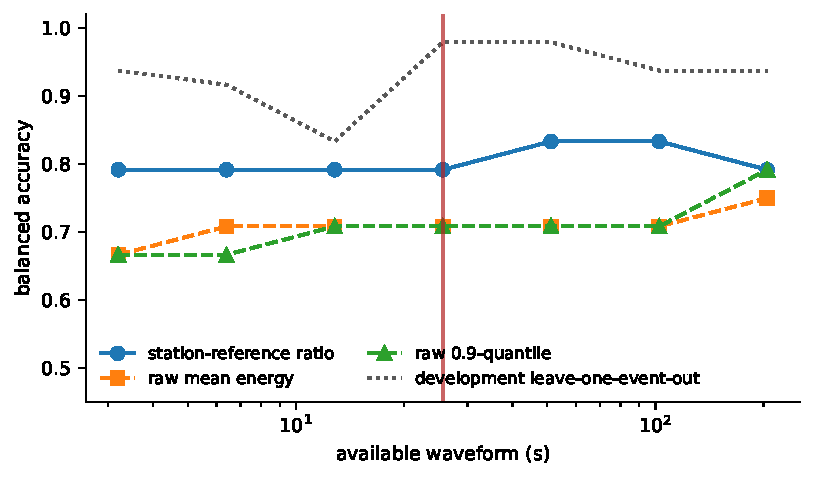
\includegraphics[width=\columnwidth]{code/manuscript_assets/figures/prefix_performance.pdf}
\caption{Latency--accuracy profile.  Solid and dashed curves are
confirmation balanced accuracy after thresholds are fit on development at
each prefix.  The dotted curve is mean leave-one-earthquake-out development
accuracy for the station-reference ratio.  The vertical line marks the
registered 25.6-second prefix.  The plot exposes both the early advantage and
the absence of monotone improvement with longer windows.}
\label{fig:prefix}
\end{figure}

Figure~\ref{fig:prefix} supplies the principal algorithmic comparison.  At
25.6 seconds, the station-reference statistic attains confirmation balanced
accuracy 0.792, while both raw controls attain 0.708.  Longer acquisition
does not uniformly improve the result.  At 204.8 seconds, the three methods
reach 0.792, 0.750, and 0.792, respectively.  The selected short prefix is
therefore not a cropped view of a superior full-window result.

\section{Confirmation results}

Table~\ref{tab:metrics} reports the fixed-prefix result.  The proposed method
improves specificity by 0.334 relative to each raw control but reduces
sensitivity by 0.166.  All three scores have the same AUC, 0.833; the gain in
balanced accuracy arises from development-threshold transfer, not from a
better ranking of every confirmation trace.

\begin{table}[H]
\centering
\caption{Confirmation performance after 25.6 seconds.  BA denotes balanced
accuracy; Sens. and Spec. denote sensitivity and specificity.}
\label{tab:metrics}
\small
\begin{tabular}{@{}lrrrr@{}}
\toprule
Method & BA & Sens. & Spec. & AUC \\
\midrule
Station-reference ratio & 0.792 & 0.667 & 0.917 & 0.833 \\
Raw mean energy          & 0.708 & 0.833 & 0.583 & 0.833 \\
Raw 0.9-quantile         & 0.708 & 0.833 & 0.583 & 0.833 \\
\bottomrule
\end{tabular}
\end{table}

The paired difference between the proposed statistic and the raw
0.9-quantile is 0.083.  Its bootstrap mean is 0.085 and its 95 percent
percentile interval is $[-0.083,0.250]$.  The interval includes zero.  The
finite confirmation supports a measured trade between false alarms and
misses but does not establish a population-level superiority claim.

\begin{figure}[H]
\centering
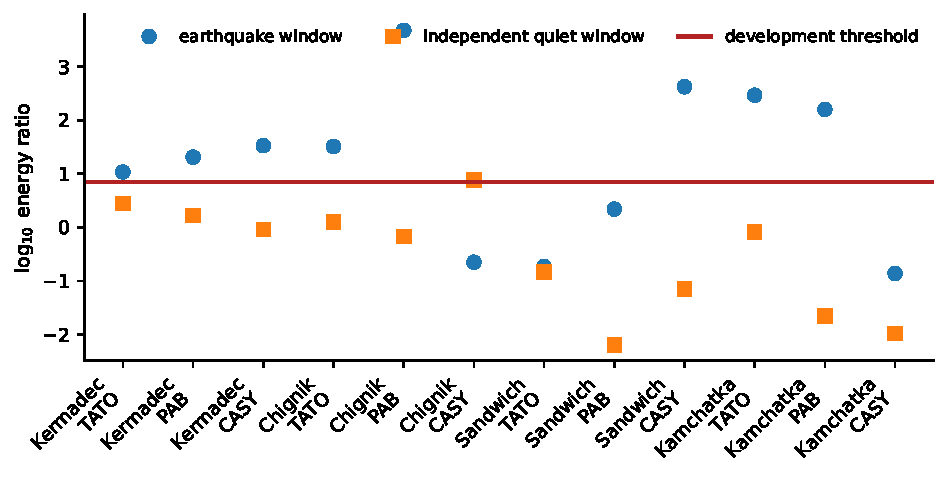
\includegraphics[width=\columnwidth]{code/manuscript_assets/figures/confirmation_scores.pdf}
\caption{All confirmation scores at the registered prefix.  Each column is
one station--earthquake pair.  Earthquake and independent quiet windows share
the one-day reference but never share candidate samples.  The horizontal line
is the development threshold.  Four event scores fall below it and one quiet
score rises above it; these failures remain visible.}
\label{fig:scores}
\end{figure}

The score plot localizes the errors.  The missed event windows occur for
Chignik at CASY, South Sandwich at TATO and PAB, and Kamchatka at CASY; the
quiet false alarm occurs for Chignik at CASY.
These outcomes are consistent with a simple amplitude-ratio statistic:
station normalization reduces broad scale mismatch but cannot compensate for
arrival geometry, propagation, or an atypical reference day.

\subsection{Runtime and storage}

Runtime is measured on the authentic Kermadec--TATO confirmation trace using
the same block-update implementation that produces the statistic.  Each
prefix is repeated 1,500 times within seven timing groups.  Figure~\ref{fig:cost}
shows the median and central 80 percent timing interval.  At eight blocks the
median is 56.1 microseconds.  At 64 blocks it is 439 microseconds, consistent
with the linear factor in Theorem~4.

\begin{figure}[H]
\centering
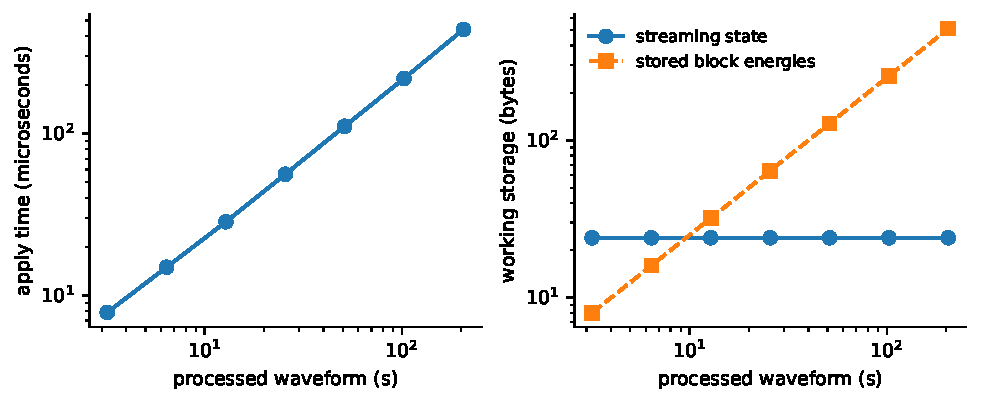
\includegraphics[width=\columnwidth]{code/manuscript_assets/figures/runtime_memory.pdf}
\caption{Computational consequence of Theorem~4.  Left: median apply time on
an authentic three-component trace; the shaded interval spans timing
quantiles 0.1--0.9.  Right: numerical state beyond the current input block.
The streaming implementation keeps three scalar state values, represented as
24 bytes, whereas retaining one float64 energy per block grows linearly.
Interpreter-object overhead and the immutable input buffer are excluded from
the storage curves.}
\label{fig:cost}
\end{figure}

The constant-state curve is an implementation contract rather than a claim
of lower wall time than optimized compiled routines.  The reference mean is
computed once from the historical trace.  Subsequent candidate processing
uses additions, multiplications, and a single logarithm at the reporting
point; no covariance formation, factorization, matrix storage, or spectral
transform is required.

\section{Scope and limitations}

The experiment has four principal limitations.  First, catalog windows are
not analyst phase picks, and the fixed 15-minute offset does not define an
operational arrival-time problem.  Second, twelve independent confirmation
pairs are sufficient to reveal failure modes but insufficient for a narrow
uncertainty interval.  Third, a one-day reference can itself be atypical;
multiple historical days and a robust reference estimator may improve
transfer but are outside the locked design.  Fourth, common-gain invariance
does not imply invariance to frequency response, orientation error, clipping,
missing channels, or temporally varying noise.

The development study was redesigned after the earlier covariance experiment
failed.  The new confirmation set was acquired only after the prefix rule and
statistic were fixed.  Its four missed event windows, one quiet false alarm,
and uncertainty interval remain in the result.  No confirmation-driven
variant replaces the locked method.

The theorem figures serve distinct purposes.  Figure~\ref{fig:scores} shows
observed distances from the decision boundary associated with the
perturbation corollary.  Figure~\ref{fig:cost} shows time and state scaling
associated with the complexity theorem.  Neither plot proves its theorem;
the equations do.  Conversely, the theorems do not guarantee the empirical
balanced accuracy in Figure~\ref{fig:prefix}.

\section{Reproducibility}

The installable package under \texttt{code/} contains the parser, frozen URL
constructors, checksums, statistic, tests, registered study, CSV tables, and
figure generator.  The offline command
\begin{center}
\small
\texttt{station-energy-study -{}-offline -{}-verify}
\end{center}
rechecks every cached payload, reruns development selection and confirmation,
regenerates all tables and figures, and compares the semantic result hash.
The locked hash is
\begin{center}
\small
\texttt{6121bb9eaa0affe7f9b3fb7e5973e5522}\allowbreak
\texttt{60f180f8c4a13e2b86042ebad93c655}.
\end{center}
Timing fields are recorded but excluded from semantic equality.  Unit tests
check batch--streaming equivalence, common-gain invariance, the sharp
perturbation bound, threshold behavior, parsing, resampling, and the retained
linear-algebra routines.  NumPy and Matplotlib provide the numerical and
plotting layers \cite{harris2020numpy,hunter2007matplotlib}.

\section{Conclusion}

Station-referenced streaming energy replaces an unsuccessful covariance
compression with a simpler physical statistic.  The method is invariant to a
common gain, admits a sharp log-ratio error certificate, and uses linear time
with constant numerical state.  On a checksum-verified confirmation set of
four later earthquakes at three new stations, it improves fixed-threshold
balanced accuracy from 0.708 to 0.792 after 25.6 seconds, chiefly by reducing
false alarms.  The paired uncertainty interval includes zero, four event
windows are missed, and the ranking AUC is unchanged.  These facts delimit the
claim: the contribution is a reproducible early-screening statistic and its
analysis, not a universal seismic detector.

\section*{Data and code availability}

Source code, frozen request metadata, SHA-256 digests, result tables, and
figure scripts are included under \texttt{code/}.  Original IU waveforms
remain at EarthScope and are downloaded from the registered FDSN URLs.  USGS
event identifiers remain resolvable through ComCat.  The repository does not
redistribute provider waveforms.

\begingroup
\small
\bibliographystyle{plainnat}
\bibliography{code/manuscript_assets/references}
\endgroup

\end{document}
